%pdflatex trans.tex
%convert -density 150x150 trans.pdf trans.png
\documentclass[border={2pt 2pt 2pt 2pt}]{standalone}
\usepackage{tikz}
\usetikzlibrary{calc}
\begin{document}

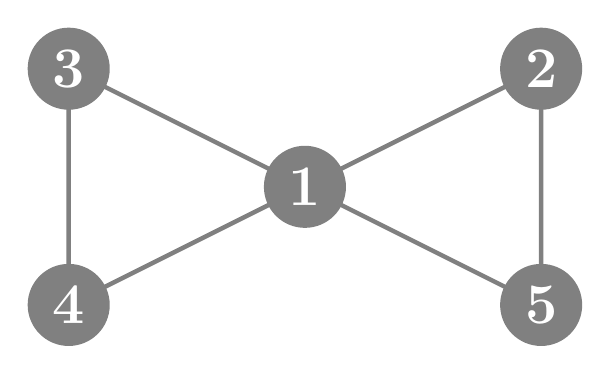
\begin{tikzpicture}
\coordinate (A) at (3,0);
\coordinate (B) at (6,1.5);
\coordinate (C) at (0,1.5);
\coordinate (D) at (0,-1.5);
\coordinate (E) at (6,-1.5);
\draw[gray,ultra thick] (A)--(B)--(E)--cycle (A)--(C)--(D)--cycle;
\draw[gray,very thick,fill=gray] (A) circle [radius=0.5];
\draw[gray,very thick,fill=gray] (B) circle [radius=0.5];
\draw[gray,very thick,fill=gray] (C) circle [radius=0.5];
\draw[gray,very thick,fill=gray] (D) circle [radius=0.5];
\draw[gray,very thick,fill=gray] (E) circle [radius=0.5];
\node[white] at (A) {\huge\bf 1};
\node[white] at (B) {\huge\bf 2};
\node[white] at (C) {\huge\bf 3};
\node[white] at (D) {\huge\bf 4};
\node[white] at (E) {\huge\bf 5};
\end{tikzpicture}

\end{document}
